% !TEX root = sn1604_wifes.tex

\begin{figure*}[tb!]
   \centering
   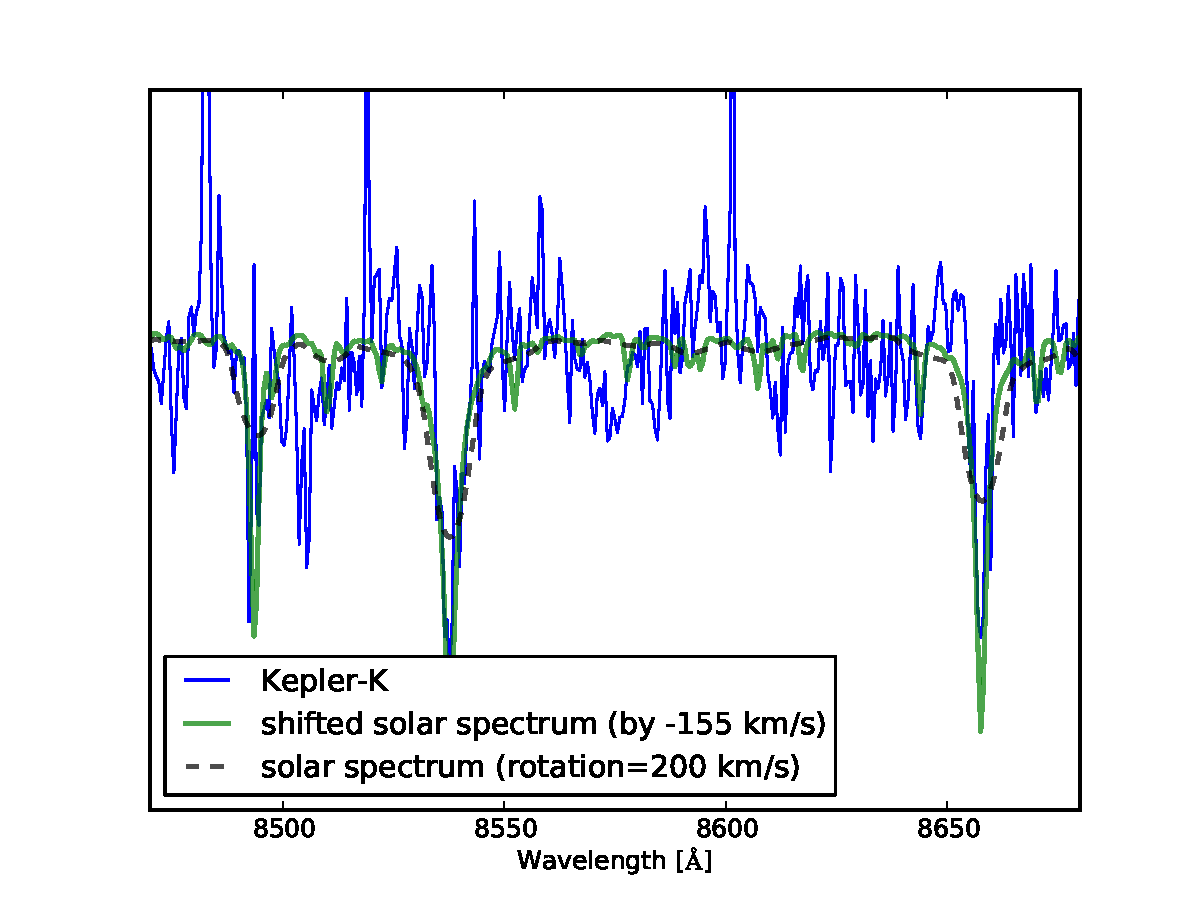
\includegraphics[width=\textwidth]{\plotdir /kepler-k-comparison.pdf} 

   \caption{The Kepler-K candidate showing a radial velocity of -155~\kms.  Such a velocity is consistent with that expected of more than a  third of the donor stars of the Kepler-SNR, but also of 5\% of unassociated stars in the direction of the remnant. Given that this study has analysed 24 stars' radial velocities, this velocity is not, on its own, indicative of an unusual star.}
   \label{fig:kepler-g}
\end{figure*}


